\mode<article>{\section{RTG-SLAM}} \mode<presentation>{\subsection{RTG-SLAM}}

\mode<article>{\subsection{Overview}}
\begin{frame}
	\mode<presentation>{\Frametitle{Overview}}
	Figure~\ref{fig:rtg-slam-overview} is the framework figure in RTG-SLAM~\autocite{peng_rtg-slam_2024}.
	\begin{figure}[htbp]
		\centering
		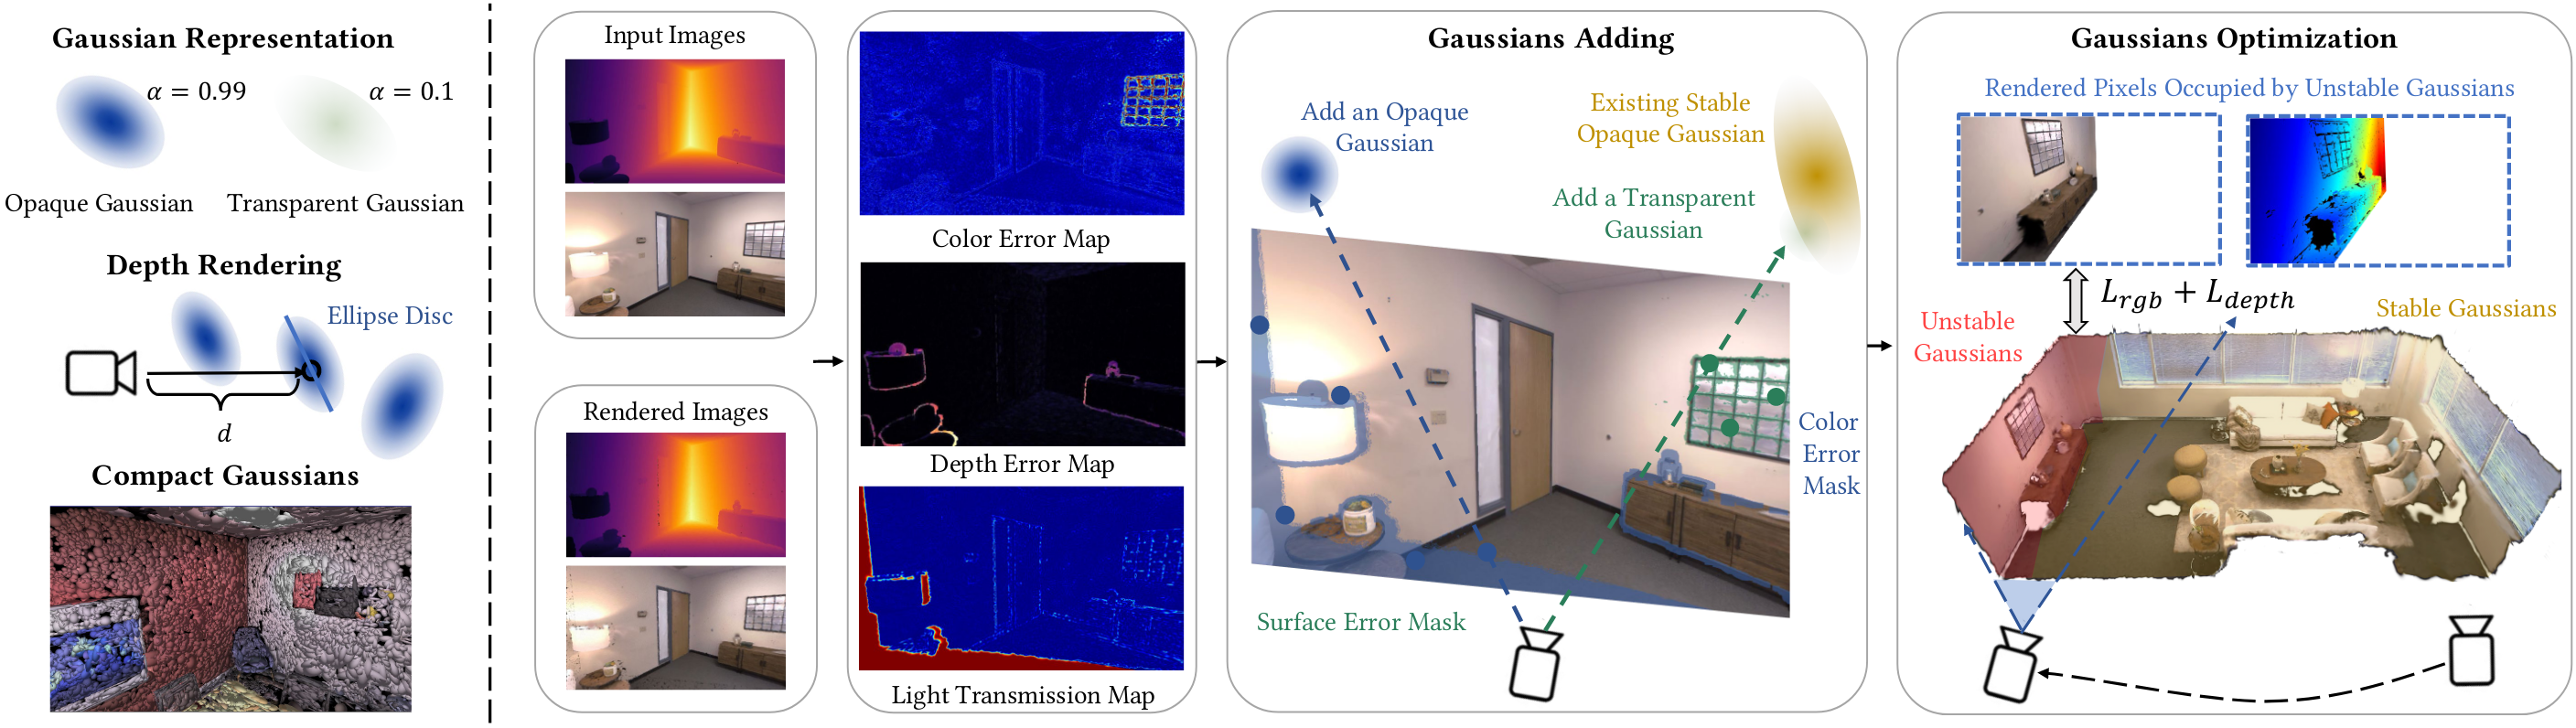
\includegraphics[width=\linewidth]{rtg-slam-overview.png}
		\smallskip
		\caption{Overview of RTG-SLAM~\autocite{peng_rtg-slam_2024}}
		\label{fig:rtg-slam-overview}
	\end{figure}
	\mode<presentation>{\blfootnote{\href{http://arxiv.org/abs/2404.19706}{(SIGGRAPH 2024) RTG-SLAM: Real-time 3D Reconstruction at Scale using Gaussian Splatting}}}
\end{frame}

\mode<article>{\subsection{Differentiable Rendering}}
\mode<article>{\subsubsection{Compact Gaussian Representation}}
\begin{frame}\mode<presentation>{\Frametitle{Compact Gaussian Representation}}
	\mode<presentation>{\blfootnote{\href{http://arxiv.org/abs/2404.19706}{(SIGGRAPH 2024) RTG-SLAM: Real-time 3D Reconstruction at Scale using Gaussian Splatting}}}
	\mode<article>{
		\par The \alert{compact} 3D Gaussian-based scene representation in RTG-SLAM~\autocite{peng_rtg-slam_2024} can be denoted by equation~\ref{eq:rtg-slam-compact-gaussian}, where the attributes that differ from the original 3D Gaussian representation~\autocite{kerbl3Dgaussians} (equation~\ref{eq:3dgs-representation}) are annotated colorfully.
	}
	\begin{block}{Compact Gaussian Representation}
		\resetcolorseries[5]{marknode-color-series}
		\resetcolorseries[5]{annotation-color-series}
		\colorlet{marknode-convention}{black!20}
		\colorlet{annotation-convention}{black}
		\begin{equation}
			\label{eq:rtg-slam-compact-gaussian}
			\tikzmarknode{n-convention-0}{\colorbox{marknode-convention}{\(\mathcal{S}\)}}  = \left\{ \mathcal{G}_i \vert i = 0,1,\cdots,N \right\}
			,\text{ where }
			\mathcal{G}_i = \left\{
			\tikzmarknode{n-convention-1}{\colorbox{marknode-convention}{\(\mathbf{p}\)}},
			\tikzmarknode{n-convention-2}{\colorbox{marknode-convention}{\(\mathbf{q}\)}},
			\tikzmarknode{n-convention-3}{\colorbox{marknode-convention}{\(\mathbf{s}\)}},
			\tikzmarknode{n-convention-4}{\colorbox{marknode-convention}{\(\mathbf{c}\)}},
			\tikzmarknode{n0}{\colorbox{marknode-color-series!![0]}{\(\alpha\)}},
			\tikzmarknode{n1}{\colorbox{marknode-color-series!![1]}{\(\mathbf{n}\)}},
			\tikzmarknode{n2}{\colorbox{marknode-color-series!![2]}{\(\eta\)}},
			\tikzmarknode{n3}{\colorbox{marknode-color-series!![3]}{\(t\)}}
			\right\}
		\end{equation}
		\begin{annotatedEquationEnv}
			\annotatedEquation{color}{n-convention-0}{south}{0em}{-1em}{north west}{annotation-convention}{scene}{east}
			\annotatedEquation{color}{n-convention-1}{south}{0em}{-1em}{north east}{annotation-convention}{\(\in \mathbb{R}^3\), position (mean)}{west}
			\annotatedEquation{color}{n-convention-2}{south}{0em}{-2em}{north east}{annotation-convention}{\(\in \mathrm{SO}(3)\), rotation (component of covariance)}{west}
			\annotatedEquation{color}{n-convention-3}{south}{0em}{-3.5em}{north east}{annotation-convention}{\(\in \mathbb{R}^3\), scale (component of covariance)}{west}
			\annotatedEquation{color}{n-convention-4}{south}{0em}{-4.75em}{north east}{annotation-convention}{\(\in \mathbb{R}^{3n}\), color (spherical harmonics)}{west}
			\annotatedEquation{colorseries}{n0}{south}{0em}{-6em}{north east}{annotation-color-series}{\(\in\{0.99,0.1\}\), ``boolean'' opacity}{west}
			\annotatedEquation{colorseries}{n1}{south}{0em}{-7.25em}{north east}{annotation-color-series}{\(\in \mathbb{R}^3\), normal vector}{west}
			\annotatedEquation{colorseries}{n2}{south}{0em}{-8.25em}{north east}{annotation-color-series}{\(\in (0,1)\), confidence}{west}
			\annotatedEquation{colorseries}{n3}{south}{0em}{-9.75em}{north east}{annotation-color-series}{\(\in \mathbb{R}\), initialization timestamp}{west}
		\end{annotatedEquationEnv}
		\vspace*{9.75em}
	\end{block}
	\mode<article>{
		\par The core of compactness is the simplified opacity. The Gaussians are forced to be either \alert{opaque} to fit the geometry and dominant color or \alert<all>{nearly transparent} to fit the residual color.
		\par The Gaussians are treated as surfel as well. \(\mathbf{n}\) is defined as the direction of the smallest eigenvector of covariance.
	}
\end{frame}

\mode<article>{\subsubsection{Appearance Rendering}}
\begin{frame}<all>[c]
	\mode<presentation>{\Frametitle{Appearance Rendering}}
	\mode<article>{
		\par The appearance rendering pipeline (RGB image) is essentially the same as described in section~\ref{sec:3dgs-rendering-pipeline} of the original 3DGS~\autocite{kerbl3Dgaussians}, except for the accelerated alpha-blending with alpha forced to be \(1\).
	}
	\mode<presentation>{\blfootnote{\href{http://arxiv.org/abs/2404.19706}{(SIGGRAPH 2024) RTG-SLAM: Real-time 3D Reconstruction at Scale using Gaussian Splatting}}}
\end{frame}

\mode<article>{\subsubsection{Geometry Rendering}}
\begin{frame}<all>[c]
	\mode<presentation>{\Frametitle{Geometry Rendering}}
	\mode<article>{
		\paragraph{Motivation} The geometry rendering pipeline (depth image) is crucial. Note that all con-current work of RTG-SLAM~\cite{peng_rtg-slam_2024} render depth in the same way as color. However, if a vanilla alpha-blending is applied for depth rendering, we can never fit a plane since limited number of Gaussians can only produce varying depth values as illustrated in figure~\ref{fig:rtg-slam-depth-rendering}.
	}
	\begin{figure}[htbp]
		\centering
		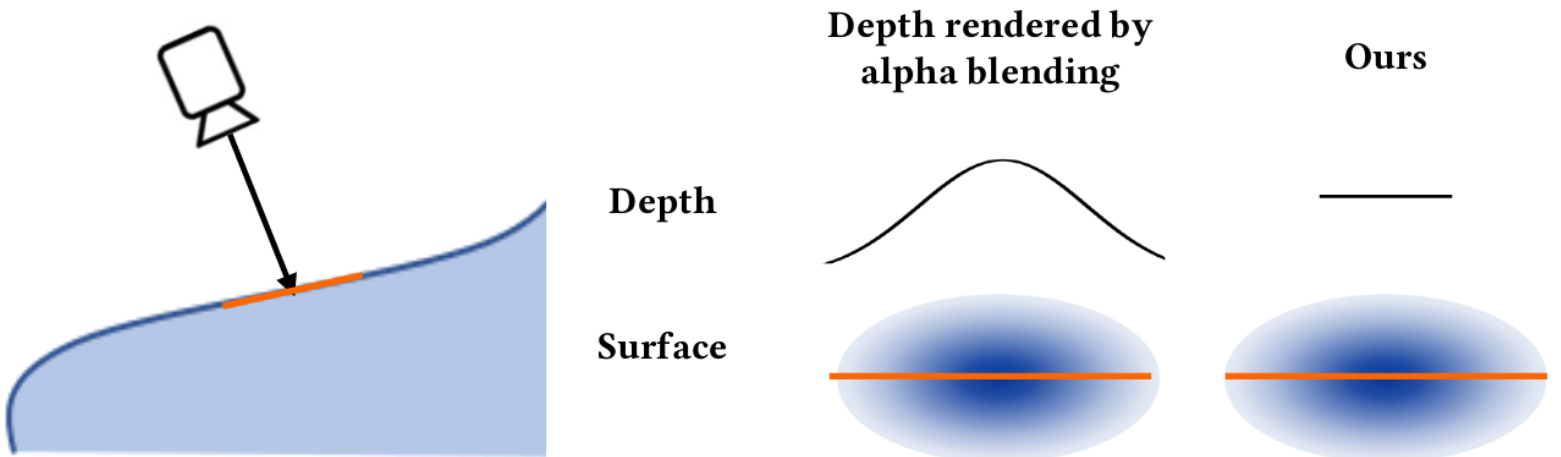
\includegraphics[width=0.6\textwidth]{rtg-slam-depth-rendering.png}
		\smallskip
		\caption{3DGS Depth Rendering: Conventional Alpha-blending v.s. RTG-SLAM}
		\label{fig:rtg-slam-depth-rendering}
	\end{figure}
	\mode<article>{
		\paragraph{Solution} In RTG-SLAM, depth images generated by 3D Gaussians are rendered in the same way as surfels.
		Fortunately, visible Gaussians are culled and front-to-back sorted in the original appearance rendering pipeline.
		\par For current camera frame and the corresponding first ``concrete''\footnote{\text{s.t. } \(\alpha > \delta_\alpha\)} Gaussian, the depth (equation~\ref{eq:rtg-slam-surfel-depth}) can be easily obtained by the ray-plane intersection formula (appendix~\ref{appendix:ray-plane-intersection}), with the ray given by equation~\ref{eq:3dgs-projection} and the plane (surfel) by equation~\ref{eq:rtg-slam-surfel}.
		\begin{block}{Surfel within Gaussian}
			\par Implicit representation of the surfel in the world coordinates.
			\resetcolorseries[5]{marknode-color-series}
			\resetcolorseries[5]{annotation-color-series}
			\begin{equation}
				\label{eq:rtg-slam-surfel}
				\left\langle
				\tikzmarknode{n0}{\colorbox{marknode-color-series!![0]}{\(\mathbf{n}\)}}
				,
				\tikzmarknode{n1}{\colorbox{marknode-color-series!![1]}{\(\mathbf{r}\)}}
				\right\rangle
				+
				\tikzmarknode{n2}{\colorbox{marknode-color-series!![2]}{\(\beta\)}}
				= 0 \text{, where }\left\langle \left(
				\tikzmarknode{n3}{\colorbox{marknode-color-series!![3]}{\(\mathbf{p}\)}}
				-
				\tikzmarknode{n4}{\colorbox{marknode-color-series!![4]}{\(\mathbf{t}\)}}
				\right), \mathbf{n} \right\rangle + \beta = 0. \\
			\end{equation}
			\vspace*{4.5em}
			\begin{annotatedEquationEnv}
				\annotatedEquation{colorseries}{n0}{south}{0em}{-0.5em}{north east}{annotation-color-series}{\(\in \mathbb{R}^{3}, \Vert \mathbf{n} \Vert = 1\),\\ normal vector of the Gaussian}{west}
				\annotatedEquation{colorseries}{n1}{south}{0em}{-3em}{north east}{annotation-color-series}{\(\in \mathbb{R}^{3}\), any point on the surfel}{west}
				\annotatedEquation{colorseries}{n2}{south}{0em}{-4.5em}{north east}{annotation-color-series}{\(\in \mathbb{R}\), offset of the surfel}{west}
				\annotatedEquation{colorseries}{n3}{south}{0em}{-2em}{north west}{annotation-color-series}{\(\in \mathbb{R}^3\), position of the Gaussian}{east}
				\annotatedEquation{colorseries}{n4}{south}{0em}{-0.5em}{north west}{annotation-color-series}{\(\in \mathbb{R}^3\), translation component of the camera's pose}{east}
			\end{annotatedEquationEnv}
		\end{block}
		\begin{equation}
			\label{eq:rtg-slam-surfel-depth}
			\theta = \frac{\langle(\mathbf{p} - \mathbf{t}) , \mathbf{n}\rangle}{\langle \mathbf{R} \mathbf{K}^{-1} \dot{\mathbf{u}}, \mathbf{n} \rangle}
		\end{equation}
		\par In practice, the rendered depth map is given by equation~\ref{eq:rtg-slam-depth-map},
		\begin{align}\label{eq:rtg-slam-depth-map}
			\hat{\mathbf{D}}\left(\mathbf{u}\right) =
			\begin{cases}
				-1,                                                                                                                                                                & \text{no intersection,}                                                                         \\[1ex]
				\displaystyle\mathbf{T}^{-1}\frac{\langle(\mathbf{p} - \mathbf{t}) , \mathbf{n}\rangle}{\langle \mathbf{R} \mathbf{K}^{-1} \dot{\mathbf{u}}, \mathbf{n} \rangle} , & \displaystyle \frac{\langle \mathbf{n}, \mathbf{r} \rangle}{\Vert \mathbf{r} \Vert} < 60^\circ, \\[2ex]
				\displaystyle\mathbf{T}^{-1}\mathbf{p}                                                                                                                             & \text{otherwise.}
			\end{cases}
		\end{align}
	}
	\mode<presentation>{\blfootnote{\href{http://arxiv.org/abs/2404.19706}{(SIGGRAPH 2024) RTG-SLAM: Real-time 3D Reconstruction at Scale using Gaussian Splatting}}}
\end{frame}

\mode<article>{\subsubsection{Others}}
\begin{frame}<all>[c]\mode<presentation>{\Frametitle{Others}}
	\par The normal map \(\hat{\mathbf{N}}\left(\mathbf{u}\right)\), the index map \(\hat{\mathbf{I}}\left(\mathbf{u}\right)\) and the transmittance map \(\hat{\mathbf{T}}\) are easily obtained by rendering pipelines, where the Gaussians' normals, indices and the light transmission are stored w.r.t pixels.
	\mode<presentation>{\blfootnote{\href{http://arxiv.org/abs/2404.19706}{(SIGGRAPH 2024) RTG-SLAM: Real-time 3D Reconstruction at Scale using Gaussian Splatting}}}
\end{frame}

\mode<article>{\subsection{Online Mapping}}
